\chapter{Grid View}
\label{sec:grid_view}

A Grid View displays DBContent data as 2-dimensional grid over two numerical variables, giving statistics over a third variable. When started, it presents itself in the following manner.

\begin{figure}[H]
    \hspace*{-2cm}
    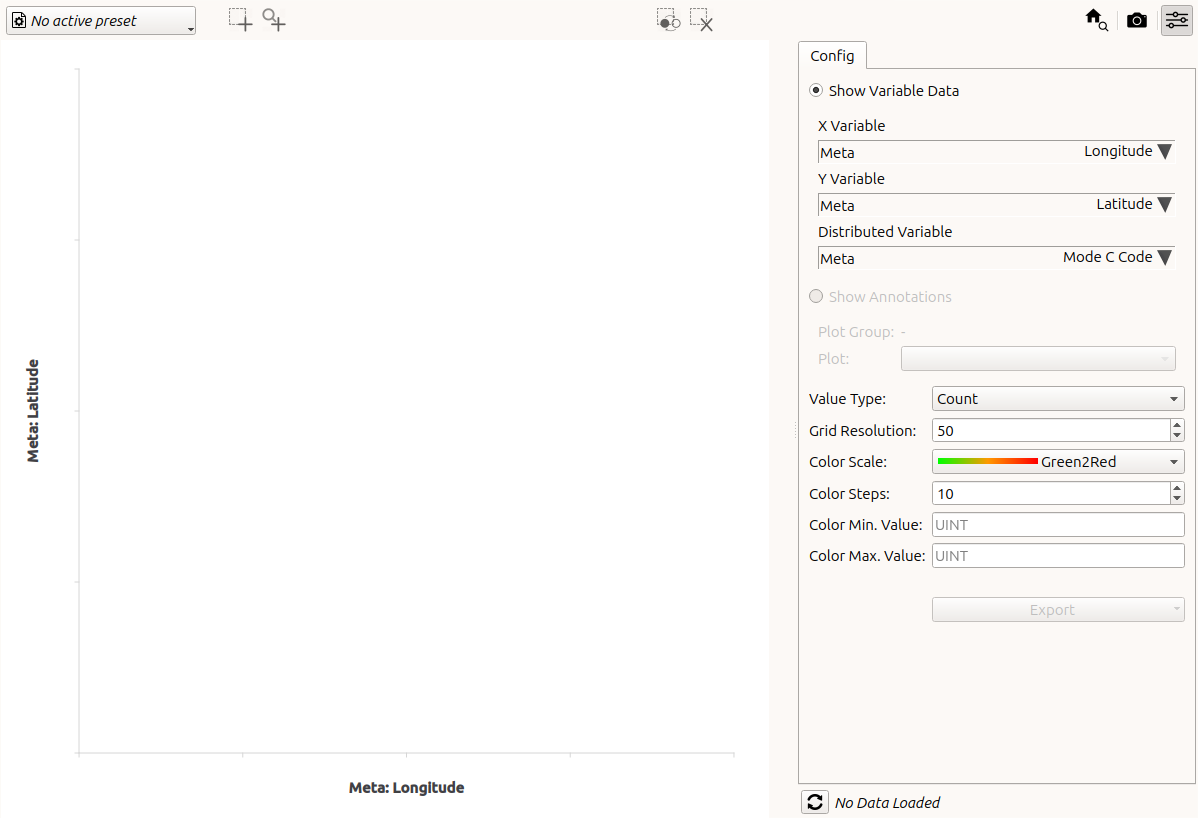
\includegraphics[width=18cm,frame]{figures/grid_start.png}
  \caption{Grid View startup}
\end{figure}

\section{Layout}

On the left side resides the plot area in which the data is visualized (if data has been loaded). The tool bar at the top shows the currently selected tool and the available actions.\\

On the right side resides the configuration area, which allows configuring what data is loaded and how it is displayed. The 'Reload' button on the bottom can be used to trigger a reload of the view's data.\\

Both areas can be resized and hidden if desired.

\section{Data Loading}

To load the data the mechanism described in Section \nameref{sec:ui_overview} or the 'Reload' button can be used. To filter the dataset, the mechanism described in Section \nameref{sec:filters} can be used. \\

\begin{figure}[H]
    \hspace*{-2cm}
    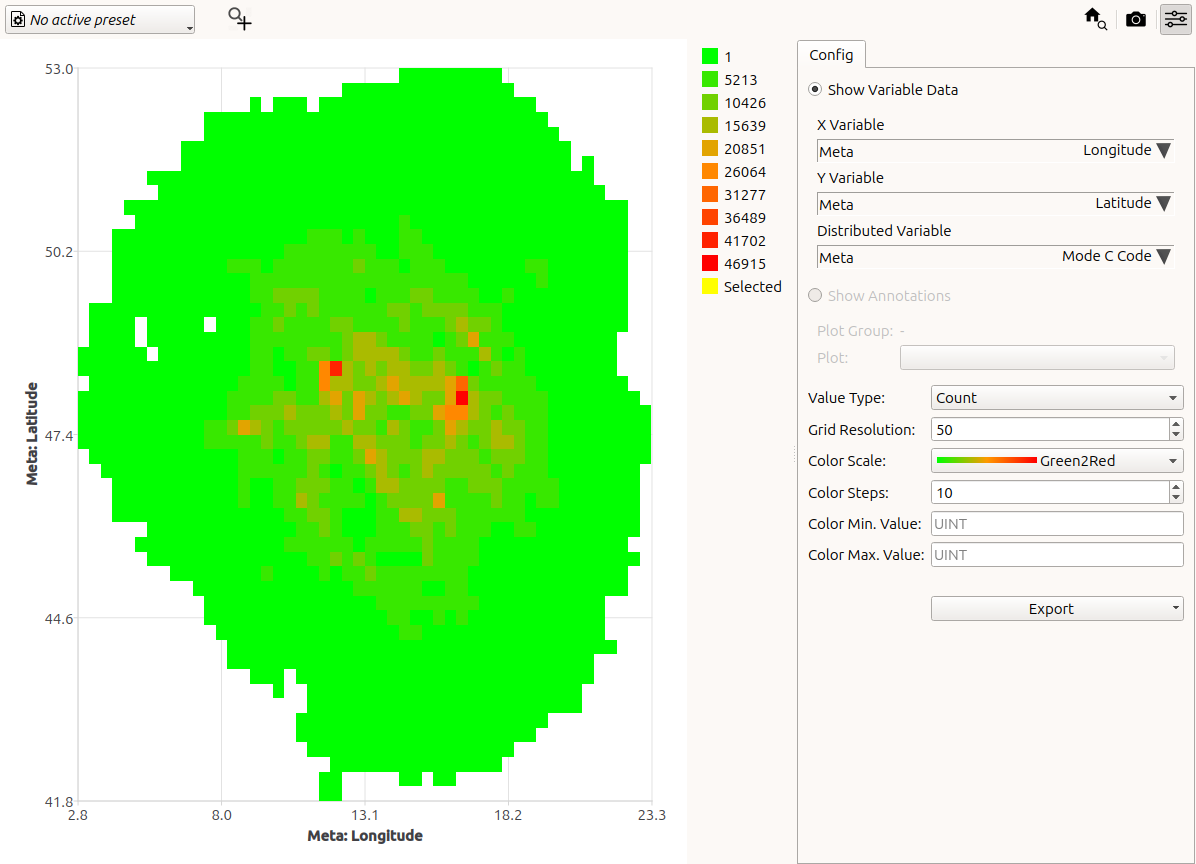
\includegraphics[width=18cm,frame]{figures/grid_loaded.png}
  \caption{Grid View after loading data}
\end{figure}

The values of the selected 'X' and 'Y' variables are used for positioning on the x-axis and y-axis.
A grid of equally spaced and sized data cells is formed over the available data range.
A third variable 'Distributed Variable' is distributed into these grid cells, each grid cell
keeping track of certain statistical values of the data sorted into it.
A single valid data point is thus formed by a value triple, and each of these values must exist in the respective DBContent. \\

The desired statistical value is extracted from each grid cell, and the grid is colored according to the extracted values. \\

Available statistical grid cell values at the moment include:

\begin{itemize}
    \item \textbf{Count}: The number of data items sorted into a grid cell
    \item \textbf{Min}: The minimum of values inside a grid cell
    \item \textbf{Max}: The maximum of values inside a grid cell
    \item \textbf{Mean}: The mean of values inside grid cell
    \item \textbf{Var}: The variance of values inside a grid cell
    \item \textbf{Stddev}: The standard deviation of values inside a grid cell
\end{itemize}
\ \\

In the current example, the meta-variable 'Mode C Code' is distributed over a grid spanned by the WGS-84 meta-variables 'Longitude' and 'Latitude'.
The data count of each grid cell is visualized, ranging from green (minimum cell data count) to red (maximum cell data count). \\

The coloring of displayed grid cells due to the visualized statistical values can be customized to the users needs. \\

On the right side of the plot a color legend is shown, describing which displayed color belongs to which value of the distributed variable.

\section{Usage}

\subsection{Toolbar}

The first buttons can be used to switch between the available tools (shortcut refers to keyboard shortcut).

Note that an active tool can always be ended by pressing the 'Escape' key.

\begin{table}[H]
  \center
  \begin{tabular}{ | l | l | l | l |}
    \hline
    \textbf{Icon} & \textbf{Shortcut} & \textbf{Text} &  \textbf{Description} \\ \hline
    %\includegraphics[width=0.5cm,frame]{../../data/icons/select_action.png} & S & Select & Allows data selection \& de-selection \\ \hline
    \includegraphics[width=0.5cm,frame]{../../data/icons/zoom_select_action.png} & R & Zoom to Rectangle & Allows zooming to the selected rectangle \\ \hline

  \end{tabular}
  \caption{Toolbar: Available tools}
\end{table}

The others provide general actions by which the view can be modified.

\begin{table}[H]
  \center
  \begin{tabular}{ | l | l | l | l |}
    \hline
    \textbf{Icon} & \textbf{Shortcut} &\textbf{Text} &  \textbf{Description} \\ \hline
    %\includegraphics[width=0.5cm,frame]{../../data/icons/select_invert.png} & & Invert Selection & Selects all de-selected \& vice versa \\ \hline
    %\includegraphics[width=0.5cm,frame]{../../data/icons/select_delete.png} & & Delete Selection & De-selects all target reports \\ \hline
    \includegraphics[width=0.5cm,frame]{../../data/icons/zoom_home.png} & Space & Zoom to Home & Pans/zooms to show all existing data \\ \hline
  \end{tabular}
  \caption{Toolbar: Available actions}
\end{table}

\subsection{Config Tab}

The selection controls on the top define which data variables are used to generate data points to be distributed over the grid.
The 'X' and 'Y' variables are used to determine the overall grid and the location of the grid cell a data point belongs to,
the 'Distributed Variable' represents the values sorted into the grid cells.
In all three cases such a variable can be any numerical variable. A reload operation might be required for the selection to take effect. \\

If available, plottable grid data of active View Points can be visualized by checking the 'Show Annotations' box.
If multiple grid annotations are present in a View Point, these individual plots can be selected using the 'Plot' combo box.
Plottable annotations might further be grouped into so-called plot groups, which are listed under 'Plot Group'.
The plot group can be switched in case multiple plot groups are available. \\

Below the variable selection, several parameters can be used to further configure the displayed grid.

\begin{itemize}
    \item \textbf{Value Type}: The statistical grid cell value to be displayed.
    \item \textbf{Grid Resolution}: The number of grid cells displayed, both in X- and Y-direction. 
    \item \textbf{Color Scale}: The color scheme used for colorization of grid cells.
    \item \textbf{Color Steps}: Number of discrete colors used for colorization of grid cells.
    \item \textbf{Color Min. Value}: The value the lower end of the color scale is assigned to. 
        If not set, the minimum of all distributed values will be chosen.
        If empty, a clue about the needed value format is shown (e.g. DOUBLE). 
    \item \textbf{Color Max. Value}: The value the upper end of the color scale is assigned to. 
        If not set, the maximum of all distributed values will be chosen.
        If empty, a clue about the needed value format is shown (e.g. DOUBLE). 
   \end{itemize}
   \ \\

\textit{Example}: The following example illustrates how the coloring can be adjusted using minimum and maximum color limits. \\

\begin{figure}[H]
    \hspace*{-2cm}
    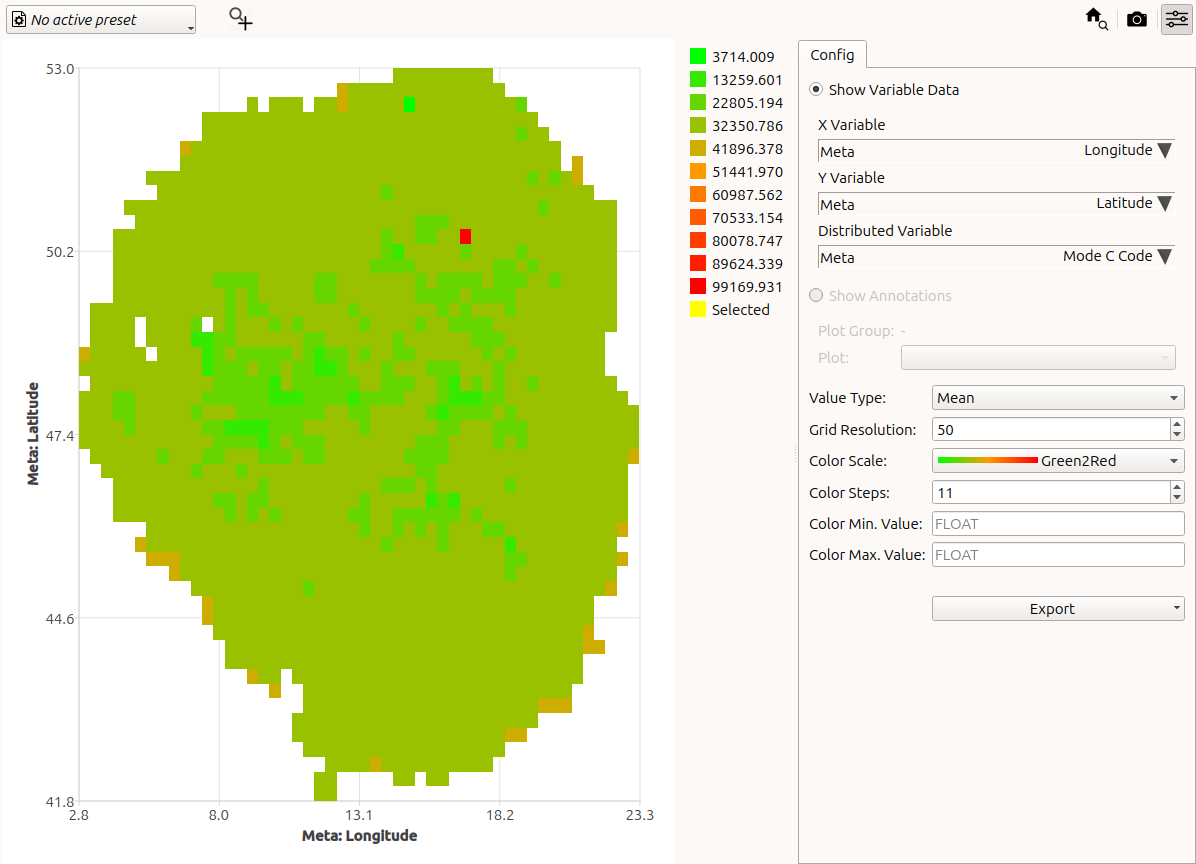
\includegraphics[width=18cm,frame]{figures/grid_modec_mean_nolimits.png}
  \caption{Grid View showing the mean Mode C Code per grid cell}
  \label{fig:grid_view_color_example1}
\end{figure}

Figure \ref{fig:grid_view_color_example1} shows a grid view which displays the mean Mode C Code of each grid cell.
No color limit values are set, so the minimum color of the chosen color scale (green) is assigned to the minimum 
value of all distributed ModeC codes, which according to the color legend is 3714.009. 
The maximum color of the chosen color scale (red) is assigned to the maximum 
value of all distributed ModeC codes, which according to the color legend is 99169.931. \\

Due to a very high maximum value, most of the grid colors are not well-separated in color.
In such a case the minimum and maximum color limits can be used to rescale the used colors
between custom values. The 'Color Min. Value' and 'Color Max. Value' parameters in figure \ref{fig:grid_view_color_example1}
show that the mean of the variable 'Mode C Code' demands a floating point value (FLOAT). 

\begin{figure}[H]
    \hspace*{-2cm}
    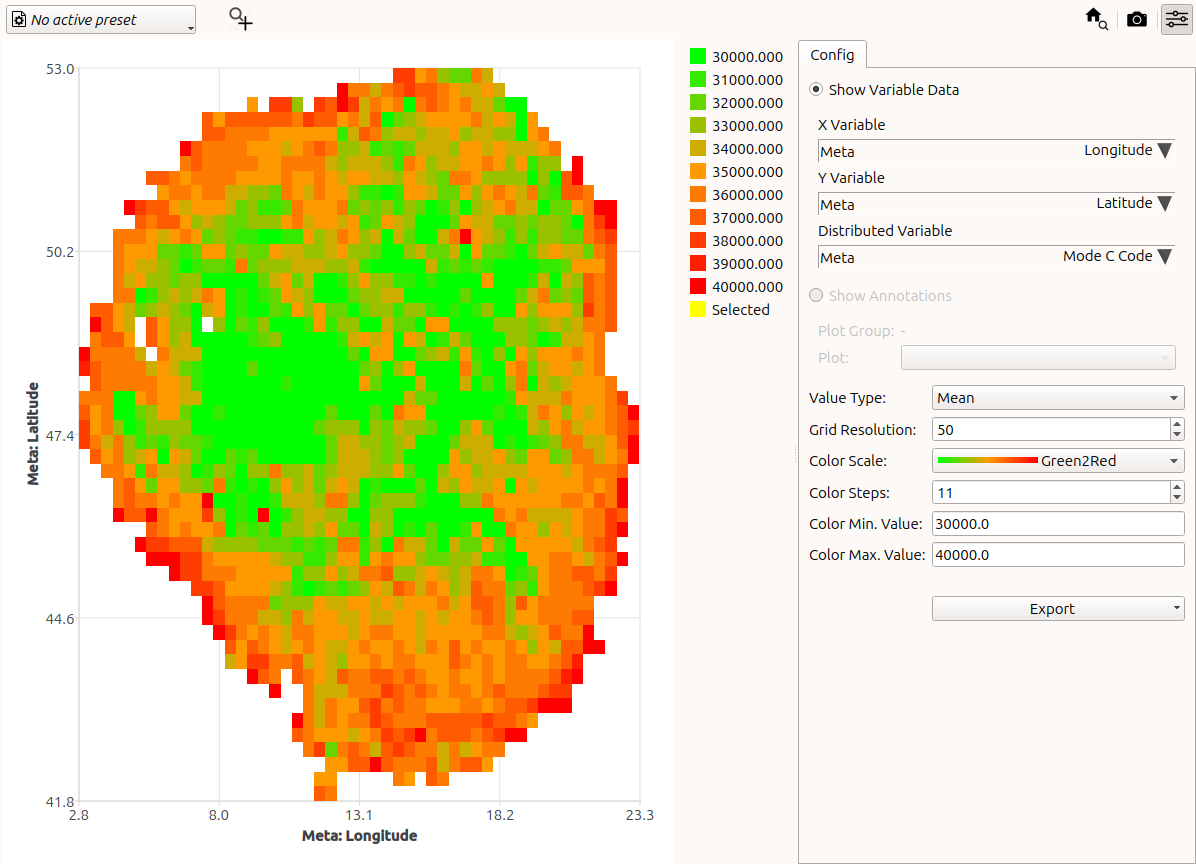
\includegraphics[width=18cm,frame]{figures/grid_modec_mean_limits.png}
  \caption{Grid View showing the mean Mode C Code per grid cell with active color limits}
  \label{fig:grid_view_color_example2}
\end{figure}

In figure \ref{fig:grid_view_color_example2} the minimum and maximum color limit were set to custom values.
The color legend shows that the color values are now scaled between 30000 (green) and 40000 (red),
which results in a better color resolution in this range.

\subsection{Export}

At the bottom of the config tab resides the export button, which is only active if the grid view is configured as follows:

\begin{itemize}
    \item The chosen X-variable is 'Meta - Longitude' 
    \item The chosen Y-variable is 'Meta - Latitude'
    \item Valid grid data is displayed
\end{itemize}

In this case the grid data can be exported by clicking on the 'Export' button and choosing the type of export. \\

\subsubsection{Export to Geographic View}
\label{sec:grid_export_geographic}

If this option is chosen, a dialog opens, which prompts the user to select the Geographic View to export the grid into and 
select a name for the exported grid item.

\begin{figure}[H]
    \center
    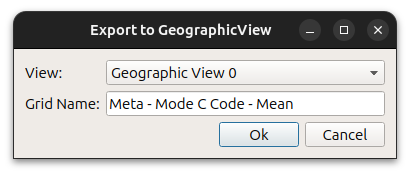
\includegraphics[width=6cm,frame]{figures/grid_export_geographic.png}
  \caption{Exporting grids to Geographic View}
\end{figure}

The grid will be exported to the selected Geographic View, and listed under \textit{Annotations}$\rightarrow$\textit{Grids} in Geographic View's 'Layers' tab.
Refer to section \ref{sec:geo_annotation_ops} for how to handle grid items in GeographicView.

\subsubsection{Export to GeoTIFF}

After choosing a filename, the grid will be exported to a GeoTIFF file, which can be imported in external software (e.g. QGIS).

%\subsection{Scatterplot}

% \subsubsection{Selection Tool}

% If the 'Select' tool is active, data can be selected. Using the left mouse-button a red selection rectangle can be spanned across all data points that should be selected.

% \begin{figure}[H]
%     \hspace*{-2cm}
%     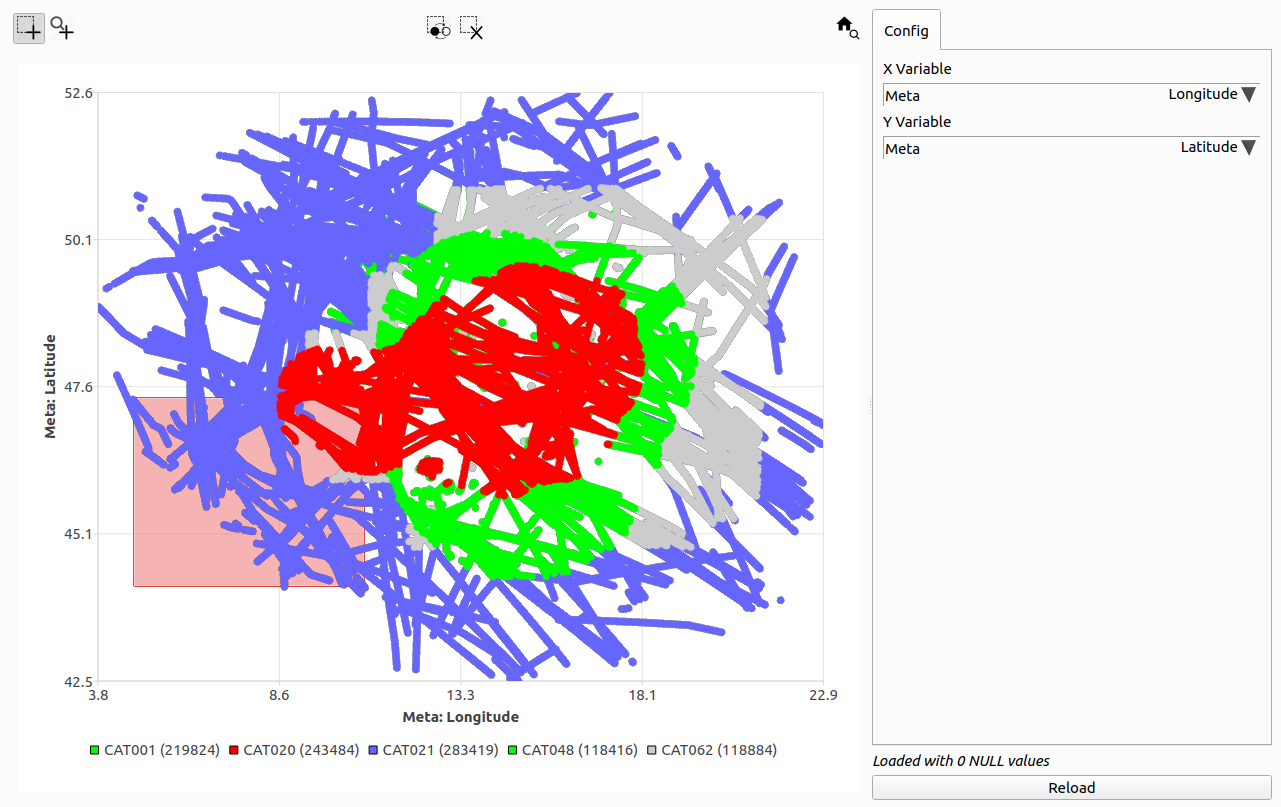
\includegraphics[width=18cm,frame]{figures/scatter_select.png}
%   \caption{Scatterplot View data selection}
% \end{figure}

% The selected data is then presented in an extra 'Selected' item in the scatter data list.

% \begin{figure}[H]
%     \hspace*{-2cm}
%     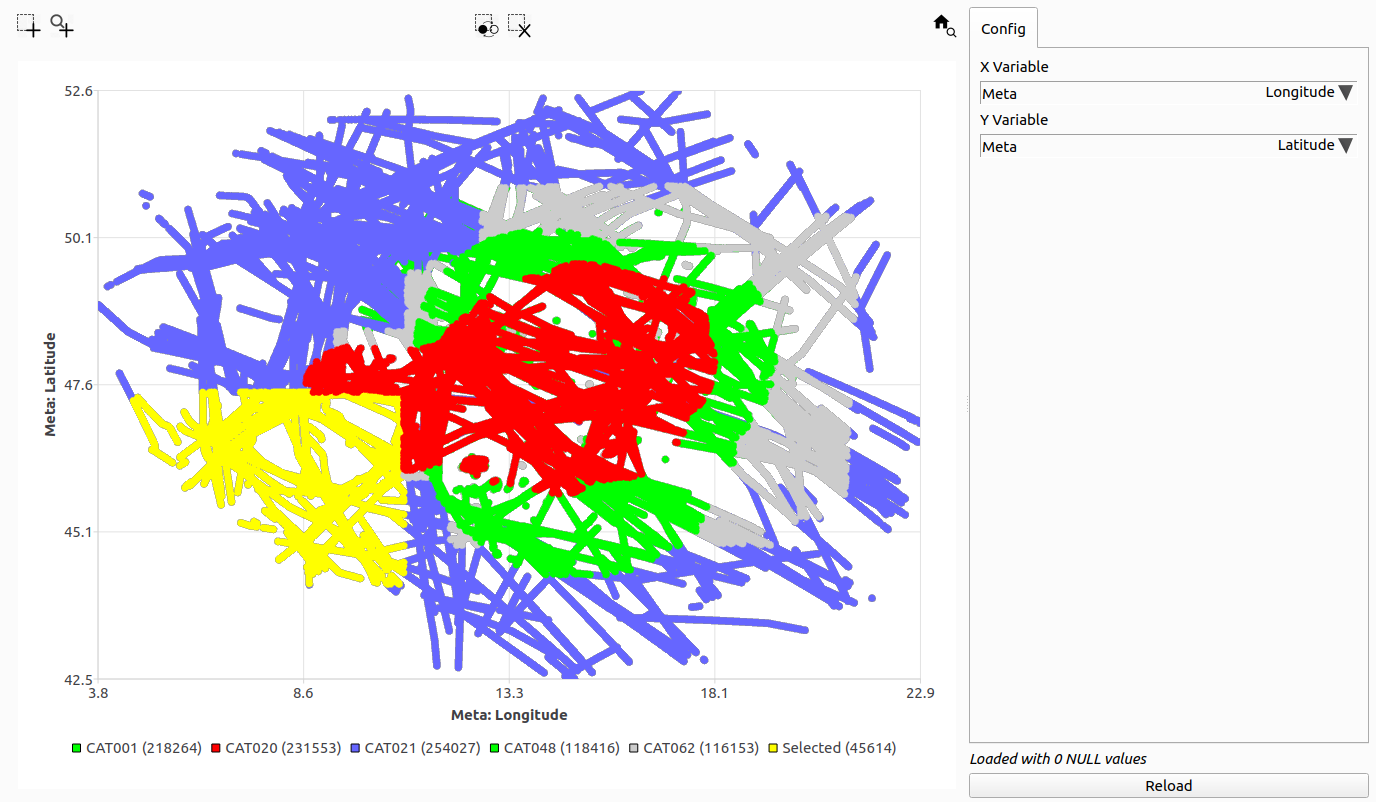
\includegraphics[width=18cm,frame]{figures/scatter_selected.png}
%   \caption{Scatterplot View data selected}
% \end{figure}

% This enables selection of parts of the data based on the presented variables, allowing deeper analysis e.g. of dubious data. \\

% %TODO_V7 maybe easier selection is the wrong term when talking about removing the selection?
% %TODO_V7 lets discuss when we talk of 'points'/'data points' and 'target reports', this is mixed up a little at the moment
% The 'Invert Selection' \includegraphics[width=0.5cm,frame]{../../data/icons/select_invert.png} or 'Delete Selection' \includegraphics[width=0.5cm,frame]{../../data/icons/select_delete.png} actions
% allow for easier selection of the wanted target reports. \\

% By pressing the 'Control' key while selecting, the newly selected data is added to any previous selection. This can be used to select data incrementally, making more complex selections possible.

\subsection{Zoom to Rectangle Tool}

Using the 'Zoom to Rectangle' tool, the left mouse-button can be used to select a rectangular region, to which a zoom operation is performed. \\

\subsection{General Zoom}

The mouse wheel can be used to zoom in or out of the presented data, the 'Space' key can be used to reset to the default zoom level (equivalent to \includegraphics[width=0.5cm,frame]{../../data/icons/zoom_home.png}).
